\documentclass{exam}

\usepackage[margin=1in]{geometry} 
\usepackage{amsmath,amsthm,amssymb, graphicx, multicol, array}
\usepackage{xcolor}
\usepackage{titling}
\usepackage{blindtext}
\usepackage{wrapfig}
\usepackage{algorithm}
\usepackage{algpseudocode}
\usepackage{float}
\usepackage{url,hyperref}

\date{}

\title{EN.525.611: Modern Convex Optimization \\
	Assignment 13 (40pts) \\
    Trajectory Optimization of Linearized Cartpole Dynamics }

% Write your name here, along with the names of any students you collaborated with.
\author{Jonathan Gill}

\begin{document}
\maketitle

\begin{multicols}{2}
\section{Introduction}
The goal of trajectory optimization is to figure out what control input should be applied to a system in a \textit{single instantaneous} state in order to achieve some desired final state subject to constraints and a desire to minimize some metric. Contrast this with a \textit{control law}, where the goal is to determine an offline policy to control a dynamical system for \textit{any} configuration that it might be in.\par

This project uses convex optimization techniques to control the linearized dynamics of an underactuated cartpole system to achieve a user-specified final system state with minimal control effort, which is a flavor of trajectory optimization. Generic trajectory optimization can be written as a nonlinear program (NLP):

\begin{equation}
    \label{traj_opt_nlp}
    \begin{aligned}
        \min_{z_{[0:N]}, u_{[0:N]}} \quad & f(z_{[0:N]}, u_{[0:N]}) \\
        \textrm{s.t.} \quad & z_0 = z_{\textrm{init}} \\
        \quad & z_N = z_{\textrm{final}} \\
        \quad & z_{i+1} = g(z_i, u_i) ~& \forall i \in [0, N-1] \\
        \quad & h_j(u_j) \leq 0 ~& \forall j \in [0, P] \\
    \end{aligned}
\end{equation}

Where $f : \mathbb{R}^n \times \mathbb{R}^m \rightarrow \mathbb{R} $ is some metric to be minimized, $z_{[0:N]}$ represent $N + 1$ states in the time interval $[0, T]$ and $u_{[0:N]}$ represent control inputs at the same time points, $g : \mathbb{R}^n \times \mathbb{R}^m \rightarrow \mathbb{R}^n$ is an approximation of the continuous time system dynamics, and $h_j(\cdot)$ are inequality constraints on some subset of the control inputs ($P \leq N$).

\end{multicols}

\begin{figure}[H]
    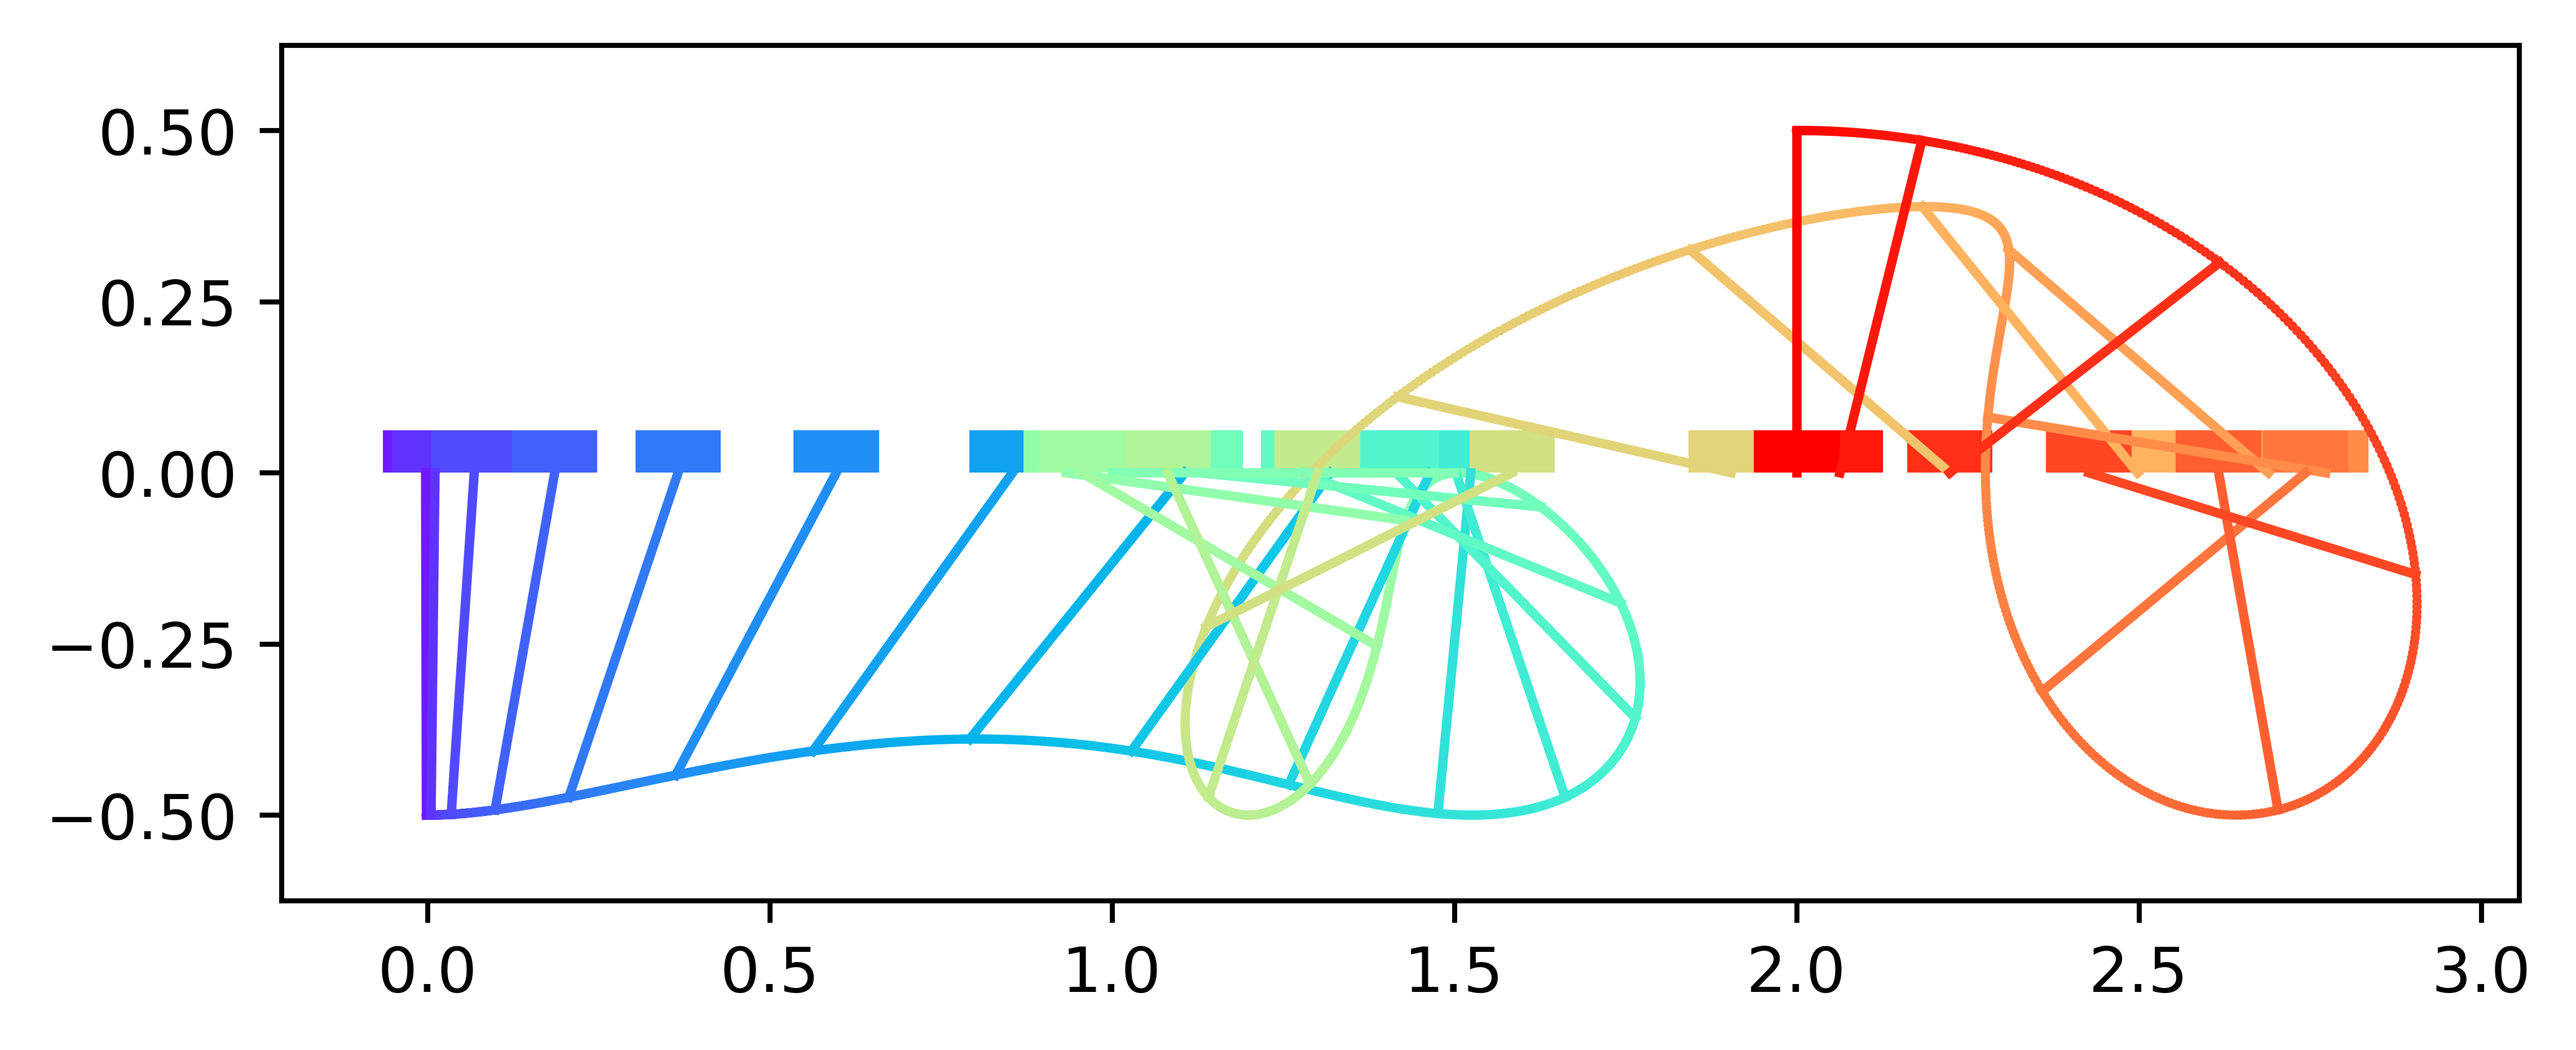
\includegraphics[width=0.9\linewidth]{cartpole_swingy.png}
    \centering
    \caption{An example of the output of trajectory optimization for a simple cartpole swing-up scenario. Purple is the initial state, red is the final state. Dynamics are linearized. The cart and pendulum arm position are shown as keyframes over the trajectory.}
    \label{fig:cartpole-swingy}
\end{figure}

\begin{multicols*}{2}

A constraint on the final state, $z_N$, is not entirely necessary and could be replaced with a penalty term in the objective function. In model predictive control applications with finite horizons, it might be best to replace the final state requirement with either a penalty on the final state or a penalty over many sequential states.

An example of an optimized trajectory is shown in Figure \ref{fig:cartpole-swingy}, where the initial state is with the cart at $(0, 0)$, pendulum hanging downward, and the final state is at $(2, 0)$ with the pendulum pointing vertically. Only lateral forces are applied to the cart.

\section{Approach}
An NLP of the form shown in \eqref{traj_opt_nlp} can be written with a quadratic objective function over $z_{[0:N]}$ and $u_{[0:N]}$ using linearized system dynamics and simple box constraints on control inputs. This formulation leads to the quadratic program shown below:

\begin{equation}
    \label{opt_prob}
    \begin{aligned}
        \min_{z_{[0:N]}, u_{[0:N]}} \quad & \frac{1}{2}\sum_{i=0}^{N} \left( z_i^T Q_i z_i + p_i^T z_i \right) + \frac{1}{2}\sum_{j=0}^N u_j^T R_j u_j \\
        \textrm{s.t.} \quad & z_0 = z_{\textrm{init}} \\
        \quad & z_N = z_{\textrm{final}} \\
        \quad & z_{i+1} = A z_i + B u_i + r_0 \quad \forall i \in [0, N-1] \\
        \quad & u_l \leq u_i \leq u_h ~\quad\quad\quad\quad\quad \forall i \in [0, N]
    \end{aligned}
\end{equation}

\begin{equation}
    \begin{aligned}
        z_i &\in \mathbb{R}^n \\
        u_i &\in \mathbb{R}^m \\
        A &\in \mathbb{R}^{n \times n} \\
        B &\in \mathbb{R}^{n \times m} \\
        r_0 &\in \mathbb{R}^n \\
        Q &\in \mathbb{R}^{n \times n} \\
        R &\in \mathbb{R}^{m \times m} \\
        N &\in \mathbb{Z_{++}} \\
        T &\in \mathbb{R_{++}}
    \end{aligned}
\end{equation}

This formulation is a convex optimization problem, which lends itself perfectly to the analyses and solution methods taught in this course. In general, the approach that this project takes to solving this optimization problem is to:

\begin{enumerate}
    \itemsep0em
    \item Use a large, finite number of elements from the matrix-exponential solution to the linearized dynamics equation to estimate $A$, $B$, and $r_0$
    \item Use the log-barrier Interior Point Method as the outer solver
    \item Rewrite \eqref{opt_prob} as a convex equality-constrained optimization problem by moving the constraints on control inputs into log barrier terms in the objective function
    \item Generate an infeasible solution by interpolating from the initial position to the final position with $u_i = 0 ~ \forall i$
    \item Use Infeasible Newton's method to determine if the initial infeasible solution \textit{can} be converted into a feasible solution
    \item Use Feasible Newton's method while increasing the log barrier strength terms until an $\epsilon$ tolerance is reached
\end{enumerate}

\section{Problem Formulation}

The following sections detail the way that elements of \eqref{opt_prob} are calculated in this project.

\subsection{Dynamics as Constraints}

A general autonomous nonlinear dynamical system can be written as

\begin{equation}
    \begin{aligned}
        \dot{z} = &f(z, u) \\
        &f : \mathbb{R}^n \times \mathbb{R}^m \rightarrow \mathbb{R}^n
    \end{aligned}
\end{equation}

which can be approximated to first-order about an arbitrary $z_0$ and $u_0$ as

\begin{equation}
    \label{linearized_dynamics}
    \begin{aligned}
        \dot{z} &= p_0 + F z + G u \\
        &= f(z_0, u_0) + \frac{\partial f(z_0, u_0)}{\partial z} (z - z_0) + \frac{\partial f(z_0, u_0)}{\partial u} (u - u_0) \\
        &= f(z_0, u_0) + \nabla_z f(z_0, u_0)^T (z - z_0) + \nabla_u f(z_0, u_0)^T (u - u_0) .
    \end{aligned}
\end{equation}

The matrices $F$ and $G$ and the vector $p_0$ are defined as the following:

\begin{equation}
    \label{eq:lin-dyn-labeled-derivs-whatevs}
    \begin{aligned}
        F &= \frac{\partial f(z_0, u_0)}{\partial z} \\
        G &= \frac{\partial f(z_0, u_0)}{\partial u} \\
        p_0 &= f(z_0, u_0) - F z_0 - G u_0
    \end{aligned}
\end{equation}

The $A$ and $B$ matrices in \eqref{opt_prob} come from the analytical solution to \eqref{linearized_dynamics} for piecewise linear control input over a fixed timestep. The general solution to \eqref{linearized_dynamics} with an unknown control input is given by the following:

\begin{equation}
    \label{general_linear_soln}
    \begin{aligned}
        z(t) &= e^{F(t - t_0)}z(t_0) + e^{Ft}\int_{t_0}^t e^{-F\tau} (G u(\tau) + p_0) d\tau \\
        &= \Phi(t, t_0)z(t_0) + \int_{t_0}^t \Phi(\tau, t_0) (G u(\tau) + p_0) d\tau
    \end{aligned}
\end{equation}

Where $\Phi(t, t_0)$ is the state transition matrix. When $u(t)$ is a constant $u_0$ over the time interval $[t_0, t_0 + \Delta t]$, the integral in \eqref{general_linear_soln} can be written as (assuming $F$ is invertible):

\begin{equation}
    \label{constant_input_integ_soln}
    \begin{split}
    &\int_{t_0}^{t_0 + \Delta t} \Phi(\tau, t_0) (G u(\tau) + p_0) d\tau\\
    &= \int_{t_0}^{t_0 + \Delta t} e^{F(t_0 + \Delta t -\tau)} (G u_0 + p_0) d\tau \\
    &= (e^{F \Delta t} - \mathbb{I})F^{-1}(G u_0 + p_0)
    \end{split}
\end{equation}

If $F$ is not invertible, then the integral in \eqref{constant_input_integ_soln} can be solved using the series representation of the matrix exponential, shown below.

\begin{equation}
\begin{aligned}
    \label{constant_input_integ_soln2}
    &\int_{t_0}^{t_0 + \Delta t} e^{F(t_0 + \Delta t -\tau)} (G u_0 + p_0) d\tau \\
    &= \sum_{k=0}^\infty \int_{t_0}^{t_0 + \Delta t} \frac{(F(t_0 + \Delta t -\tau))^k}{k!} d \tau (G u_0 + p_0)\\
    &= \left( \sum_{k=1}^\infty \frac{F^{k-1} \Delta t^{k}}{k!} \right) (G u_0 + p_0) \\
    &= \left( \Delta t + \frac{F \Delta t^2}{2!} + \frac{F^2 \Delta t^3}{3!} + ... \right) (G u_0 + p_0)
    % &= e^{F \Delta t}z(t_0) + \left( \sum_{k=1}^\infty \frac{F^{k-1} \Delta t^{k}}{k!} \right) (G u_0 + p_0) \\
    % &= e^{F \Delta t}z(t_0) + \left( \Delta t + \frac{F \Delta t^2}{2!} + \frac{F^2 \Delta t^3}{3!} + ... \right) (G u_0 + p_0)
\end{aligned}
\end{equation}

The matrices $A$ and $B$ and the vector $r_0$ are short hands for the results from equations \eqref{general_linear_soln} and \eqref{constant_input_integ_soln2}:

\begin{equation}
    \begin{aligned}
        A &= e^{F \Delta t} = \sum_{k=0}^\infty \frac{(F \Delta t)^{k}}{k!} \\
        B &= \sum_{k=1}^\infty \frac{F^{k-1} \Delta t^{k}}{k!} G \\
        r_0 &= \sum_{k=1}^\infty \frac{F^{k-1} \Delta t^{k}}{k!} p_0
    \end{aligned}
\end{equation}

\subsection{Interior Point Method}

This project places no penalty on system states, only on the control effort exerted to achieve a desired final state. We also weight control effort across all timesteps uniformly. This means that the $Q_i$ matrices and $p_i$ vectors in \eqref{opt_prob} are zero and $R_j = R ~\forall j \in [0, N]$.

The inequality constraints on control input in \eqref{opt_prob} are replaced with log-barrier terms in the objective function. The maximum and minimum bounds on the control inputs are converted into the following log barrier terms

\begin{equation}
    \begin{aligned}
        \phi_h(u_i) &= - \frac{1}{t} \log(-(u_i - u_h)) \\
        \phi_l(u_i) &= - \frac{1}{t} \log(-(u_l - u_i))
    \end{aligned}
\end{equation}

Where $\phi_h$ are log barrier terms for the control input upper bound and $\phi_l$ are log barrier terms on the control input lower bound. Replacing the inequality constraints with $\phi_h$ and $\phi_l$ reduces the optimization problem in \eqref{opt_prob} to:

\begin{equation}
    \label{the_actual_opt_prob}
    \begin{aligned}
        \min_{z_{[0:N]}, u_{[0:N]}} \quad& \frac{1}{2}\sum_{j=0}^N u_j^T R u_j + \sum_{i=0}^N\phi_h(u_i) + \sum_{i=0}^N \phi_l(u_i) \\
        \textrm{s.t.} \quad& z_0 = z_{\textrm{init}} \\
        \quad & z_N = z_{\textrm{final}} \\
        \quad & z_{i+1} = A z_i + B u_i + r_0 \quad \forall i \in [0, N-1] \\
    \end{aligned}
\end{equation}

The Interior Point Method requires that all centering steps must be feasible, however, generating an initial feasible solution to this problem is difficult because of the presence of the final state constraint. Calculating an initial feasible solution amounts to finding a suboptimal trajectory for $z_{[0:N]}$ and $u_{[0:N]}$ that satisfies the linearized system dynamics defined by $A$, $B$, and $r_0$. Fortunately, Infeasible Newton's method exists to handle cases just like this.

The Interior Point Method implementation for this project proceeds as shown in algorithm \ref{ipm_alg}, where superscripts indicate a step number.

\end{multicols*}

\begin{algorithm}
\caption{Interior Point Method}
\label{ipm_alg}
\begin{algorithmic}
    \Require $T > 0$ \Comment{Duration of the trajectory)}
    \Require $N > 0$ \Comment{Number of samples along the duration of the trajectory}
    \Require $z_{[0:N]}^0$, $u_{[0:N]}^0$ \Comment{Not necessarily feasible, but with $z_0 = z_{\textrm{init}}$}
    \Require $t^0 > 1$ \Comment{Log barrier parameter}
    \Require $\mu \approx 10$ \Comment{Log barrier increase term}
    \Require $\epsilon_{\textrm{infeas}} \approx 10^{-8}$ \Comment{Termination criteria for Infeasible Newton}
    \Require $\epsilon_{\textrm{feas}} \approx 10^{-8}$ \Comment{Termination criteria for Feasible Newton}
    \Require $\alpha \in (0, 0.5]$ \Comment{Line search comparison parameter}
    \Require $\beta \in (0, 0.9]$ \Comment{Line search step-size reduction parameter}

    \State
    \State For the sake of clarity, let $Z^i = z_{[0:N]}^i$ and $U^i = u_{[0:N]}^i$ be stacks of states and control inputs, respectively
    \State $Z^1$, $U^1$, res = InfeasibleNewton($Z^0$, $U^0$, $t^0$, A, B, $r_0$, $\epsilon_{\textrm{infeas}}$, $\alpha$, $\beta$)
    \If{$||\textrm{res}||_2 > \epsilon_{\textrm{infeas}}$}
        \State \Return Problem is infeasible
    \EndIf
    \While{$\frac{m}{t} > \epsilon_{\textrm{feas}}$} \Comment{$m$ is the number of log barrier terms in the objective function}
        \State $Z^{k+1}$, $U^{k+1}$ = FeasibleNewton($Z^{k}$, $U^{k}$, $t^k$, A, B, $r_0$, $\epsilon_{\textrm{feas}}$, $\alpha$, $\beta$)
        \State $t^{k+1} \gets \beta t^k$
    \EndWhile
\end{algorithmic}
\end{algorithm}

\begin{multicols*}{2}
\subsection{Infeasible Start Newton's Method}

Infeasible Newton's method is a primal-dual method for solving equality constrained convex optimization problems of the form show in \eqref{eq_cons_opt_prob}. This method is used in this project only for the first centering step of the Interior Point Method.

\begin{equation}
    \label{eq_cons_opt_prob}
    \begin{aligned}
        \min_{x} \quad & f(x) \\
        \textrm{s.t.} \quad & Ux = w.
    \end{aligned}
\end{equation}

Where $x \in \mathbb{R}^n$ is the decision variable, $f : \mathbb{R}^n \rightarrow \mathbb{R}$ is convex, $U \in \mathbb{R}^{m \times n}$ is full row rank, and $w \in \mathbb{R}^m$. Solving the nonlinear system of equations that result from the KKT conditions of \eqref{eq_cons_opt_prob} subsequently solves the optimization problem. The problem's Lagrangian is given by $L = f(x) + \nu^T\left( Ux - w \right)$, and the subsequent KKT conditions are shown below.

\begin{equation}
    \label{eq_cons_opt_prob_kkt}
    \begin{aligned}
        \nabla_x L(x, \nu) = \nabla_x f(x^*) + U^T\nu^* &= 0 \\
        Ux^* &= w
    \end{aligned}
\end{equation}

Where $\nu$ is the unbounded dual variable associated with the equality constraints. The power of Infeasible Newton derives from the fact that an initial infeasible solution converges to a feasible solution as the problem is being optimized. Solutions to these kinds of optimization problems are found by treating the KKT conditions as a root-finding problem and using Newton's method to slowly converge to the roots. Iterates to the primal and dual variables are found by solving the following system of equations (where superscript $k$ indicates an iterate number).

\begin{equation}
    \label{infeas_newt_deltas}
    \begin{pmatrix}
        \nabla^2_x f(x^k) & U^T \\
        U & 0
    \end{pmatrix}
    \begin{pmatrix}
        \Delta x^k \\
        \Delta \nu^k
    \end{pmatrix} = 
    -\begin{pmatrix}
        \nabla_xf(x^k) + U^T \nu^k \\
        Ux^k - w
    \end{pmatrix}
\end{equation}

Where the residual vector, $r(x^k, \nu^k)$, is defined as the RHS of \eqref{infeas_newt_deltas},

\begin{equation}
    r(x^k, \nu^k) = \begin{pmatrix}
        \nabla_xf(x^k) + U^T \nu^k \\
        Ux^k - w
    \end{pmatrix}
\end{equation}

and 

\begin{equation}
    \begin{aligned}
        x^{k+1} &= x^k + s \Delta x^k \\
        \nu^{k+1} &= \nu^k + s \Delta \nu^k .
    \end{aligned}
\end{equation}

Where $s$ is a step-size determined by line search over the norm of the residual (as opposed to the objective function). Infeasible Start Newton's Method works because the \textit{residual} vector is non-increasing over a one-dimensional extrapolation from some given point $x^k, \nu^k$ in the direction of $\Delta x^k, \Delta \nu^k$ from \eqref{infeas_newt_deltas}. It's also worth noting that, because of the infeasible start, the objective function value might sometimes increase over the execution of Infeasible Start Newton's Method. The entire algorithm is shown in Algorithm \ref{infeas-start-newtons-algo}.

\end{multicols*}

\begin{algorithm}
    \caption{Infeasible Start Newton's Method}
    \label{infeas-start-newtons-algo}
    \begin{algorithmic}
        \Require $x^0 \in \textrm{dom} f, \nu \in \mathbb{R}^m, \alpha \in (0, 0.5], \beta \in (0, 1)$
        \Require $\gamma >0, \gamma \approx 10^{-8}$ \Comment{Constraint satisfaction threshold}
        \Require $\epsilon >0, \epsilon \approx 10^{-5}$ \Comment{Desired residual vector norm threshold}
        \While{$||Ux - w||_2 > \gamma$ and $||r(x^k, \nu^k)||_2 > \epsilon$}
            \State Calculate $\Delta x^k$, $\Delta \nu^k$ from Eq \eqref{infeas_newt_deltas}
            \State $s \gets 1$
            \While{$ x^k + s \Delta x^k \notin \textrm{dom} f$ or $||r(x^k + s \Delta x^k, \nu^k + s \Delta \nu^k)||_2 > (1 - \alpha s)||r(x^k, \nu^k)||_2$}
                \State $s \gets \beta s$
            \EndWhile
            \State $x^{k+1} = x^k + s \Delta x^k$
            \State $\nu^{k+1} = \nu^k + s \Delta \nu^k$
        \EndWhile
    \end{algorithmic}
\end{algorithm}

\begin{multicols}{2}
\subsection{Feasible Start Newton's Method}

After an initial feasible trajectory is generated via Infeasible Start Newton's Method the Interior Point Method implementation in this project uses Feasible Start Newton's Method to further optimize the solution while increasing the log barrier penalty terms in the objective function.

If the initial solution to the optimization problem in \eqref{eq_cons_opt_prob} is feasible, then we can solve an approximation of the original problem by letting $x \rightarrow x + \Delta x$, approximating $f(x + \Delta x)$ up to a quadratic, and requiring that $U(x + \Delta x) = w$.

\begin{equation}
    \label{feas-newt-of-approx}
    \begin{aligned}
        &f(x + \Delta x) \approx \\
        &\quad f(x) + \nabla f(x)^T \Delta x + \frac{1}{2}\Delta x^T \nabla^2f(x) \Delta x
    \end{aligned}
\end{equation}

\begin{equation}
    \label{feas-newt-eq-cons}
    \begin{aligned}
        U(x + \Delta x) &= Ux + U \Delta x = w \\
        w + U \Delta x &= w \implies U \Delta x = 0
    \end{aligned}
\end{equation}

Replacing the original optimization problem with the approximate values from \eqref{feas-newt-of-approx} and \eqref{feas-newt-eq-cons} leaves

\begin{equation}
    \label{feas-newt-approx-eq-cons-opt-prob}
    \begin{aligned}
        \min_{\Delta x} \quad & f(x) + \nabla f(x)^T \Delta x + \frac{1}{2}\Delta x^T \nabla^2f(x) \Delta x \\
        \textrm{s.t.} \quad & U\Delta x = 0.
    \end{aligned}
\end{equation}

with the KKT conditions shown below (where $\nu$ is the dual variable associated with the equality constraints).

\begin{equation}
    \label{feas-newt-kkt-conds}
    \begin{aligned}
        \nabla f(x) + \nabla^2 f(x) \Delta x + U^T\nu &= 0 \\
        U \Delta x &= 0
    \end{aligned}
\end{equation}

Similarly to Infeasible Start Newton's Method, these are rewritten as a system of linear equations, $\Delta x$ and $\Delta \nu$ are solved for, and $x^k$ and $\nu^k$ are updated using backtracking line search. The system of linear equations is

\begin{equation}
    \begin{pmatrix}
        \nabla^2 f(x^k) & U^T \\
        U & 0
    \end{pmatrix}
    \begin{pmatrix}
        \Delta x^k \\
        \Delta \nu^k
    \end{pmatrix}
    = -\begin{pmatrix}
       \nabla f(x^k) \\
       0
    \end{pmatrix}
\end{equation}

and only the primal decision variable is updated, $x^{k+1} = x^k + s \Delta x^k$, where $s$ is a step size that comes from backtracking line search. The algorithm for Feasible Start Newton's Method is shown in \ref{feas-start-newtons-algo}.

\subsection{Cartpole Dynamics}

Cartpole dynamics have been derived to death everywhere and anywhere. Figure \ref{fig:cartpole} shows a generic cartpole configuration, where $\phi$ increases in a counterclockwise direction and the cart is located exactly on the $x$-axis. The cart has mass $m_c$, the pendulum arm is massless with length $l_{p}$, and a mass $m_{p}$ is fixed to the end of the pendulum arm. The cart can be subjected to a force along the $x$-axis within the range $F_l \leq F_c \leq F_h$. The system is conservative, so neither the cart nor the pendulum experience any drag forces.

\begin{figure}[H]
    \centering
    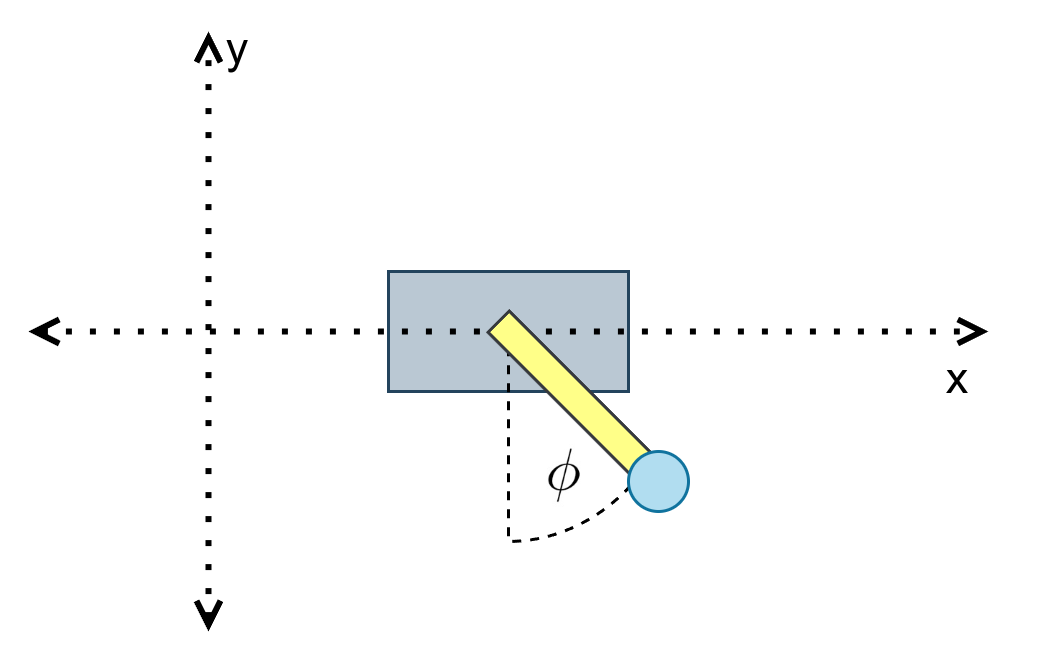
\includegraphics[width=1.0\linewidth]{cartpole.drawio.png}
    \caption{Cartpole system. The cart is constrained to move along the $x$-axis, and the pendulum makes angle $\phi$ relative to the cart's body $y$-axis.}
    \label{fig:cartpole}
\end{figure}

The undamped cartpole's system states are the cart's position and velocity, and the pendulum's angular position and angular velocity. These are arranged into a column vector, $z = [x \quad \phi \quad \dot{x} \quad \dot{\phi}]^T$. The cartpole's nonlinear equations of motion, written in terms of $z$, are shown below.

\begin{equation}
    \label{eq:nonlin-cartpole-dynamics}
    \dot{z}
    = \begin{pmatrix}
        z_3 \\
        z_4 \\
        \frac{ -g\sin{z_2}\cos{z_2} - l_p u - l_p z_4^2\sin{z_2} }{\cos^2{z_2} - l_p \alpha}\\
        \frac{ \alpha g\sin{z_2} + u\cos{z_2} + z_4^2\sin{z_2}\cos{z_2}} {\cos^2{z_2} - l_p \alpha}
    \end{pmatrix}
\end{equation}

Where $\alpha = (m_c + m_p)/(m_p l_p)$, $g$ is the constant gravity term $9.8 \textrm{m}/\textrm{s}^2$, and $F_c = u m_p l_p \in \mathbb{R}$ is a force applied to the cart.

The linearized cartpole dynamics are similarly tedious to derive, so their derivations are omitted and non-trivial entries from the $F$ and $G$ matrices from \eqref{eq:lin-dyn-labeled-derivs-whatevs} are shown below in equations \eqref{eq:f-start} - \eqref{eq:g-end}. Technically the $G$ matrix is actually a vector, $G \in \mathbb{R}^n$, since $u \in \mathbb{R}$.

For all experiments carried out in this project, the cartpole's dynamics are linearized about the point $z = [0 \quad 0 \quad 0 \quad 0]^T$.

\end{multicols}

\begin{equation}
    \label{eq:f-start}
    F_{3,2} = \frac{g \sin^{2}{\left(z_{2} \right)} - g \cos^{2}{\left(z_{2} \right)} - l z_{4}^{2} \cos{\left(z_{2} \right)}}{- \alpha l + \cos^{2}{\left(z_{2} \right)}} + \frac{2 \left(- g \sin{\left(z_{2} \right)} \cos{\left(z_{2} \right)} - l u - l z_{4}^{2} \sin{\left(z_{2} \right)}\right) \sin{\left(z_{2} \right)} \cos{\left(z_{2} \right)}}{\left(- \alpha l + \cos^{2}{\left(z_{2} \right)}\right)^{2}}
\end{equation}

\begin{equation}
    F_{3,4} = - \frac{2 l z_{4} \sin{\left(z_{2} \right)}}{- \alpha l + \cos^{2}{\left(z_{2} \right)}}
\end{equation}
%
\begin{equation}
    \begin{aligned}
        F_{4,2} &= \frac{\alpha g \cos{\left(z_{2} \right)} - u \sin{\left(z_{2} \right)} - z_{4}^{2} \sin^{2}{\left(z_{2} \right)} + z_{4}^{2} \cos^{2}{\left(z_{2} \right)}}{- \alpha l + \cos^{2}{\left(z_{2} \right)}} \\
        &+ \frac{2 \left(\alpha g \sin{\left(z_{2} \right)} + u \cos{\left(z_{2} \right)} + z_{4}^{2} \sin{\left(z_{2} \right)} \cos{\left(z_{2} \right)}\right) \sin{\left(z_{2} \right)} \cos{\left(z_{2} \right)}}{\left(- \alpha l + \cos^{2}{\left(z_{2} \right)}\right)^{2}}
    \end{aligned}
\end{equation}
%
\begin{equation}
    F_{4,4} = \frac{2 z_{4} \sin{\left(z_{2} \right)} \cos{\left(z_{2} \right)}}{- \alpha l + \cos^{2}{\left(z_{2} \right)}}
\end{equation}
%
\begin{equation}
    G_3 = - \frac{l}{- \alpha l + \cos^{2}{\left(z_{2} \right)}}
\end{equation}
%
\begin{equation}
    \label{eq:g-end}
    G_4 = \frac{\cos{\left(z_{2} \right)}}{- \alpha l + \cos^{2}{\left(z_{2} \right)}}
\end{equation}

\begin{algorithm}
    \caption{Feasible Start Newton's Method}
    \label{feas-start-newtons-algo}
    \begin{algorithmic}
        \Require $x^0 \in \textrm{dom} f, Ux^0 = w, \nu \in \mathbb{R}^m, \alpha \in (0, 0.5], \beta \in (0, 1)$
        \Require $\epsilon >0, \epsilon \approx 10^{-5}$ \Comment{Desired Newton decrement threshold}
        \While{$\lambda^2(x^k) > \epsilon$} \Comment{$\lambda^2(x^k) = (\Delta x^k)^T \nabla^2 f(x^k) \Delta x^k$}
            \State Calculate $\Delta x^k$, $\Delta \nu^k$ from Eq \eqref{infeas_newt_deltas}
            \State $s \gets 1$
            \While{$ x^k + s \Delta x^k \notin \textrm{dom} f$ or $f(x^k + s \Delta x^k) > f(x^k) + \alpha s \nabla f(x^k)^T \Delta x^k$}
                \State $s \gets \beta s$
            \EndWhile
            \State $x^{k+1} = x^k + s \Delta x^k$
            \State $\nu^{k+1} = \nu^k + s \Delta \nu^k$
        \EndWhile
    \end{algorithmic}
\end{algorithm}

\pagebreak

\begin{multicols}{2}
\subsection{Nitty gritty details}

The control input and state variables are mashed together in one primal decision variable, $x$. The first $N + 1$ entries in $x$ are the scalar control inputs, and the remaining $4 \times (N + 1)$ entries contain state variables. The primal decision variable looks like the following:

\begin{equation}
    \begin{aligned}
        x &= \begin{pmatrix}
        u_0 &
        u_1 &
        ... &
        u_N &
        z_0 &
        z_1 &
        ... &
        z_N
    \end{pmatrix}^T \\
    &= \begin{pmatrix}
        u_{[0:N]}^T &
        z_{[0:N]}^T
    \end{pmatrix}^T \in \mathbb{R}^{(S + 1)(N + 1)}
    \end{aligned}
\end{equation}

Where $S$ is the size of the state vector for the dynamical system, in this case $S = 4$. A state at some step $i$ occupies indices in the range (assuming zero-based indexing) $[N + 1 + Si, N + 1 + Si + S - 1]$ in the primal state vector, and a control input at some step $i$ occupies index $i$.

Since the control inputs and states are smashed into one variable, the matrix $R$ in \eqref{the_actual_opt_prob} is the upper-left block of a larger matrix $Q \in \mathbb{R}^{(S + 1)(N + 1) \times (S + 1)(N + 1)}$.

This project requires the Jacobian (gradient transpose) and Hessian of the objective function of the objective function from the optimization problem in \eqref{the_actual_opt_prob}. Since only the control input terms are part of the objective function, the Jacobian is non-zero in the first $(N + 1)$ elements, and the Hessian is non-zero in the upper left block of size $(N + 1) \times (N + 1)$.

The gradient of the objective function with respect to the control inputs (writing $u = u_{[0:N]}$ and $z = z_{[0:N]}$) is

\begin{equation}
    \nabla_u f (x) = Ru - \frac{1}{t}\left( \frac{1}{u - u_l} + \frac{1}{u_h - u} \right)
\end{equation}

Where $\frac{1}{v}$ is taken to mean the element-wise inverse of the vector $v \in \mathbb{R}^{n}$ and adding or subtracting a scalar from a vector is the same as subtracting the scalar value from each element of the vector.

The Hessian of the objective function with respect to the control inputs is

\begin{equation}
    \nabla^2_u f (x) = Q + \frac{1}{t}\textrm{diag}\left( \frac{1}{(u - u_l)^2} + \frac{1}{(u_h - u)^2} \right)
\end{equation}

Where $v^2$ is taken to mean a vector whose elements are squared individually, or equivalently, the Hadamard product of $v$ with itself. This project uses $Q = \mathbb{I}$, leading the Hessian to be especially sparse. This sparsity is not exploited as part of the implementation, but it certainly could be. 

The equality constraints for system dynamics, initial state, and final state are placed in one large, sparse matrix to make it easier to integrate them into the two flavors of Newton's method. The matrix $U \in \mathbb{R}^{S(N + 2) \times (S + 1)(N + 1)}$ is exceptionally sparse, but again, this sparsity is not exploited in this implementation. As an example, the dynamics constraint $z_1 = A z_0 + b u_0 + r_0$ can be rearranged as

\begin{equation}
    \begin{aligned}
        z_1 - A z_0 - b u_0 = r_0
    \end{aligned}
\end{equation}

and which can be written less conveniently using index ranges of the primal decision variable $x$ as

\begin{equation}
    \begin{aligned}
        x_{[N+1 + S: N + 1 + 2S -1]} - A x_{[N+1: N + 1 + S -1]} - b x_{[0]} = r_0
    \end{aligned}
\end{equation}

Adding dynamics constraints requires inserting $A$ matrices and $b$ vectors into specific portions of the $U$ matrix. The included Jupyter notebook has more details.

\section{Experiments}

The experiments in this project were haphazardly constructed and mostly designed to verify that implementations of complicated algorithms were working correctly (this project was mostly focused on implementation details).

That said, the core experiment was to verify that a linearized cartpole system, starting in the configuration $z_0 = [0 \quad 0 \quad 0 \quad 0]^T$, could be swung up to the final position $z_f = [* \quad \pi \quad 0 \quad 0]^T$ over a time interval $t \in [0, T]$, with some number of points along the trajectory, $N$, with control inputs in some user-defined range $u_i \in [u_l, u_h]$, exerting some minimal amount of control effort.

The result of one of these experiments is shown in Figure \ref{fig:cartpole-swingy}, where the control input is between $[-30, 30]$ over $T = 2$ seconds. The control input for this trajectory is shown in Figure \ref{fig:default-config-trajectory}.

One particularly interesting experiment is finding the minimum time required to generate a feasible trajectory to a desired final position given some input constraints. For the parameters listed above, it turns out that roughly 1.24 seconds are required to move achieve the desired final state under minimal control effort. Plots of the trajectory and control input for this configuration are included in Figure \ref{fig:shortest-time-trajectory}, note that the control inputs exhibit some characteristics of a bang-bang control system.

On the flip side, if the system is given ample time to reach the final state, the control inputs are more subdued over the duration of the trajectory. This allows the cart to slowly "wiggle" the pendulum in near-vertical configurations until the final time is achieved. It's interesting to note that the control input in \ref{fig:loooong-time-trajectory} exhibits a kind of beat-pattern. This might suggest that one high frequency and one low frequency system mode are being excited and exploited to minimize the total control effort.

\begin{figure}[H]
    \centering
    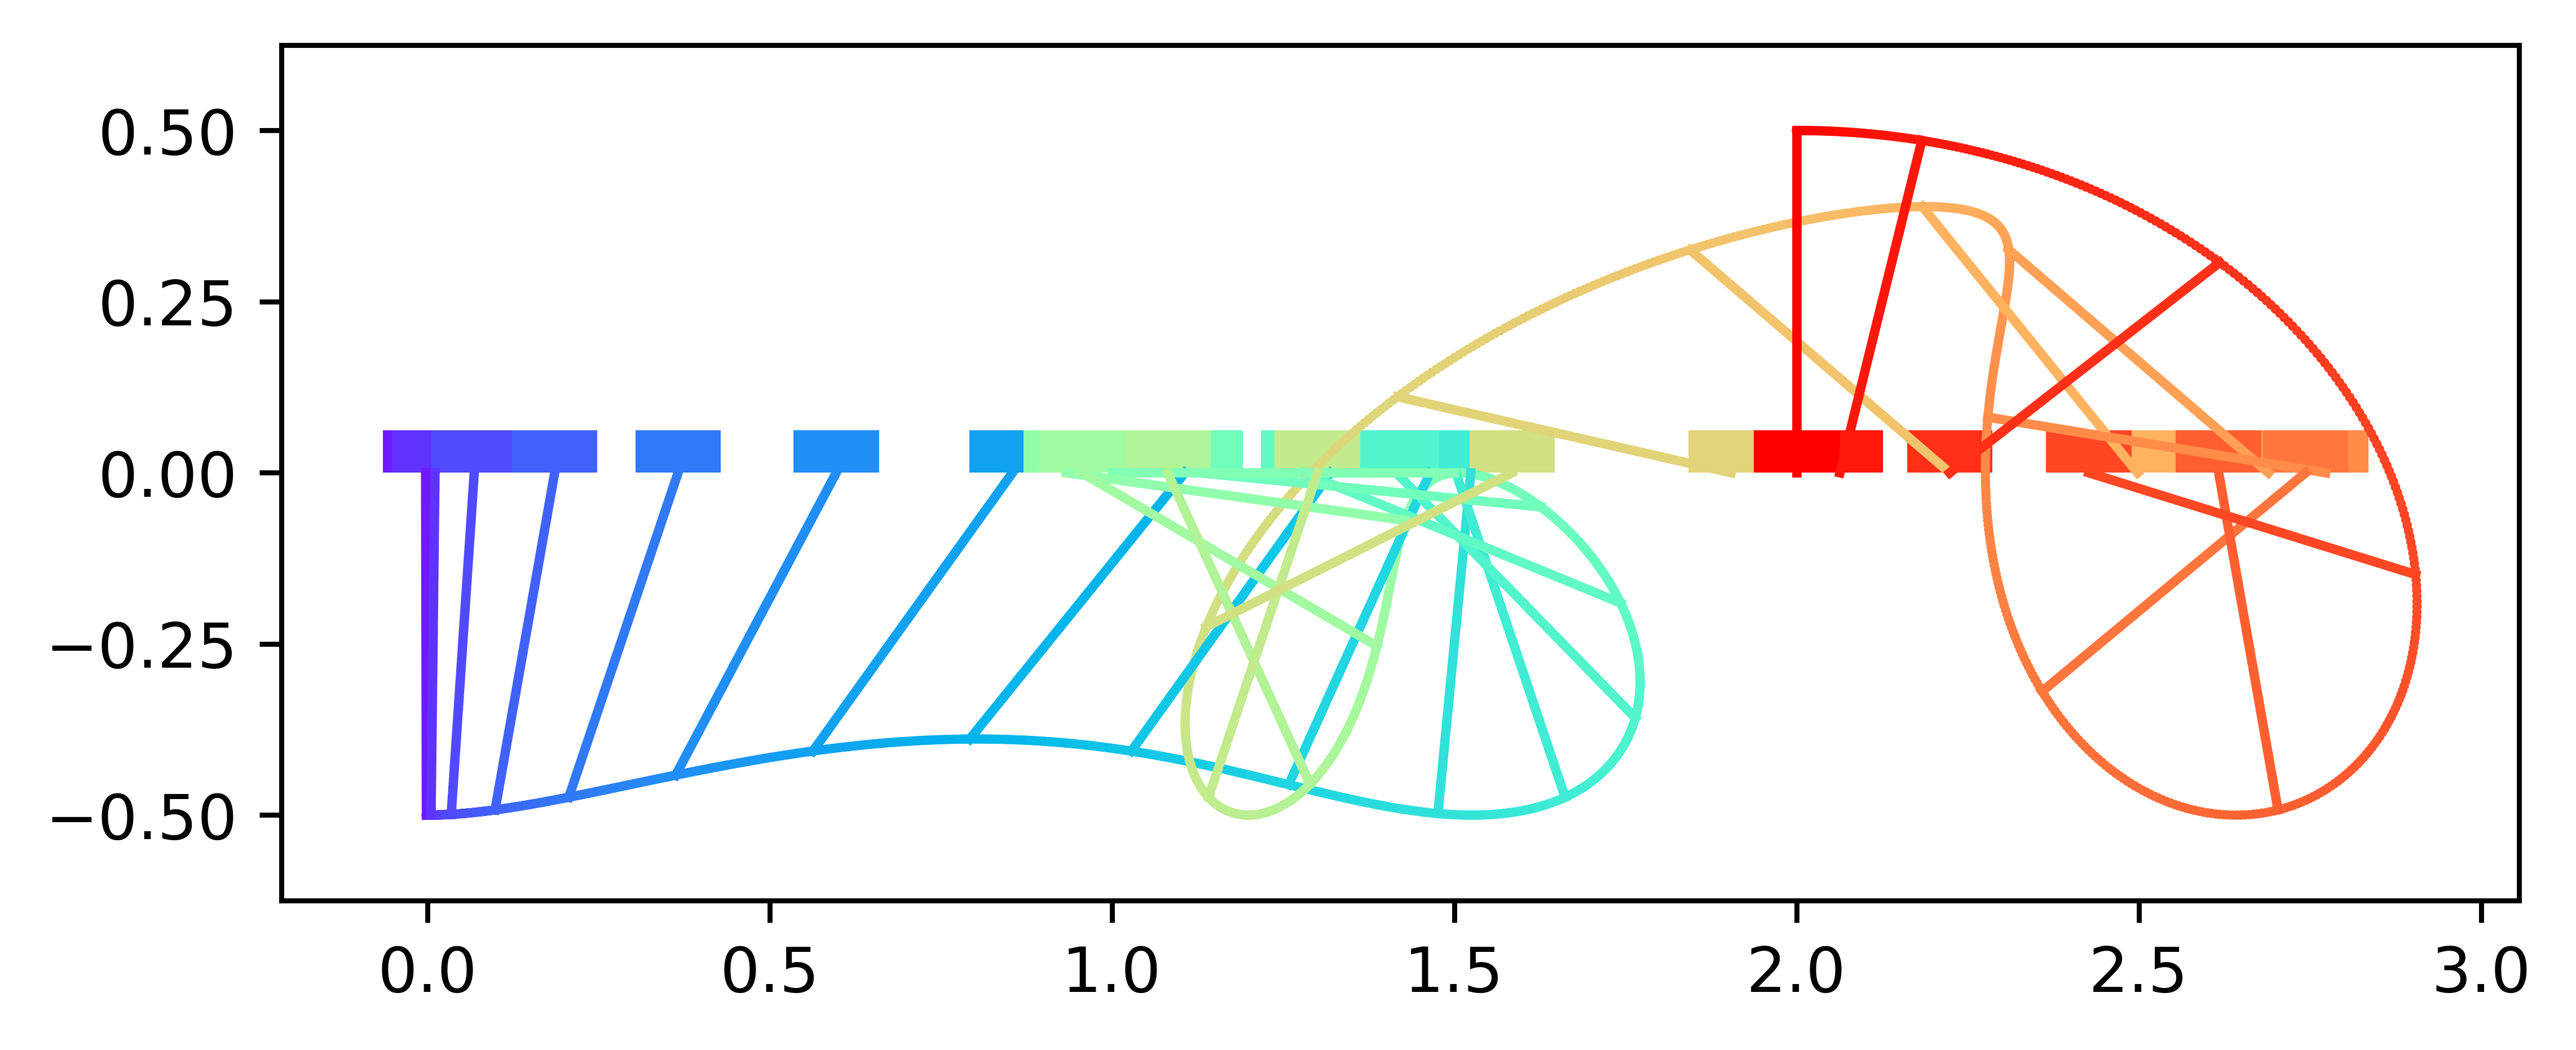
\includegraphics[width=1.0\linewidth]{cartpole_swingy.png}
    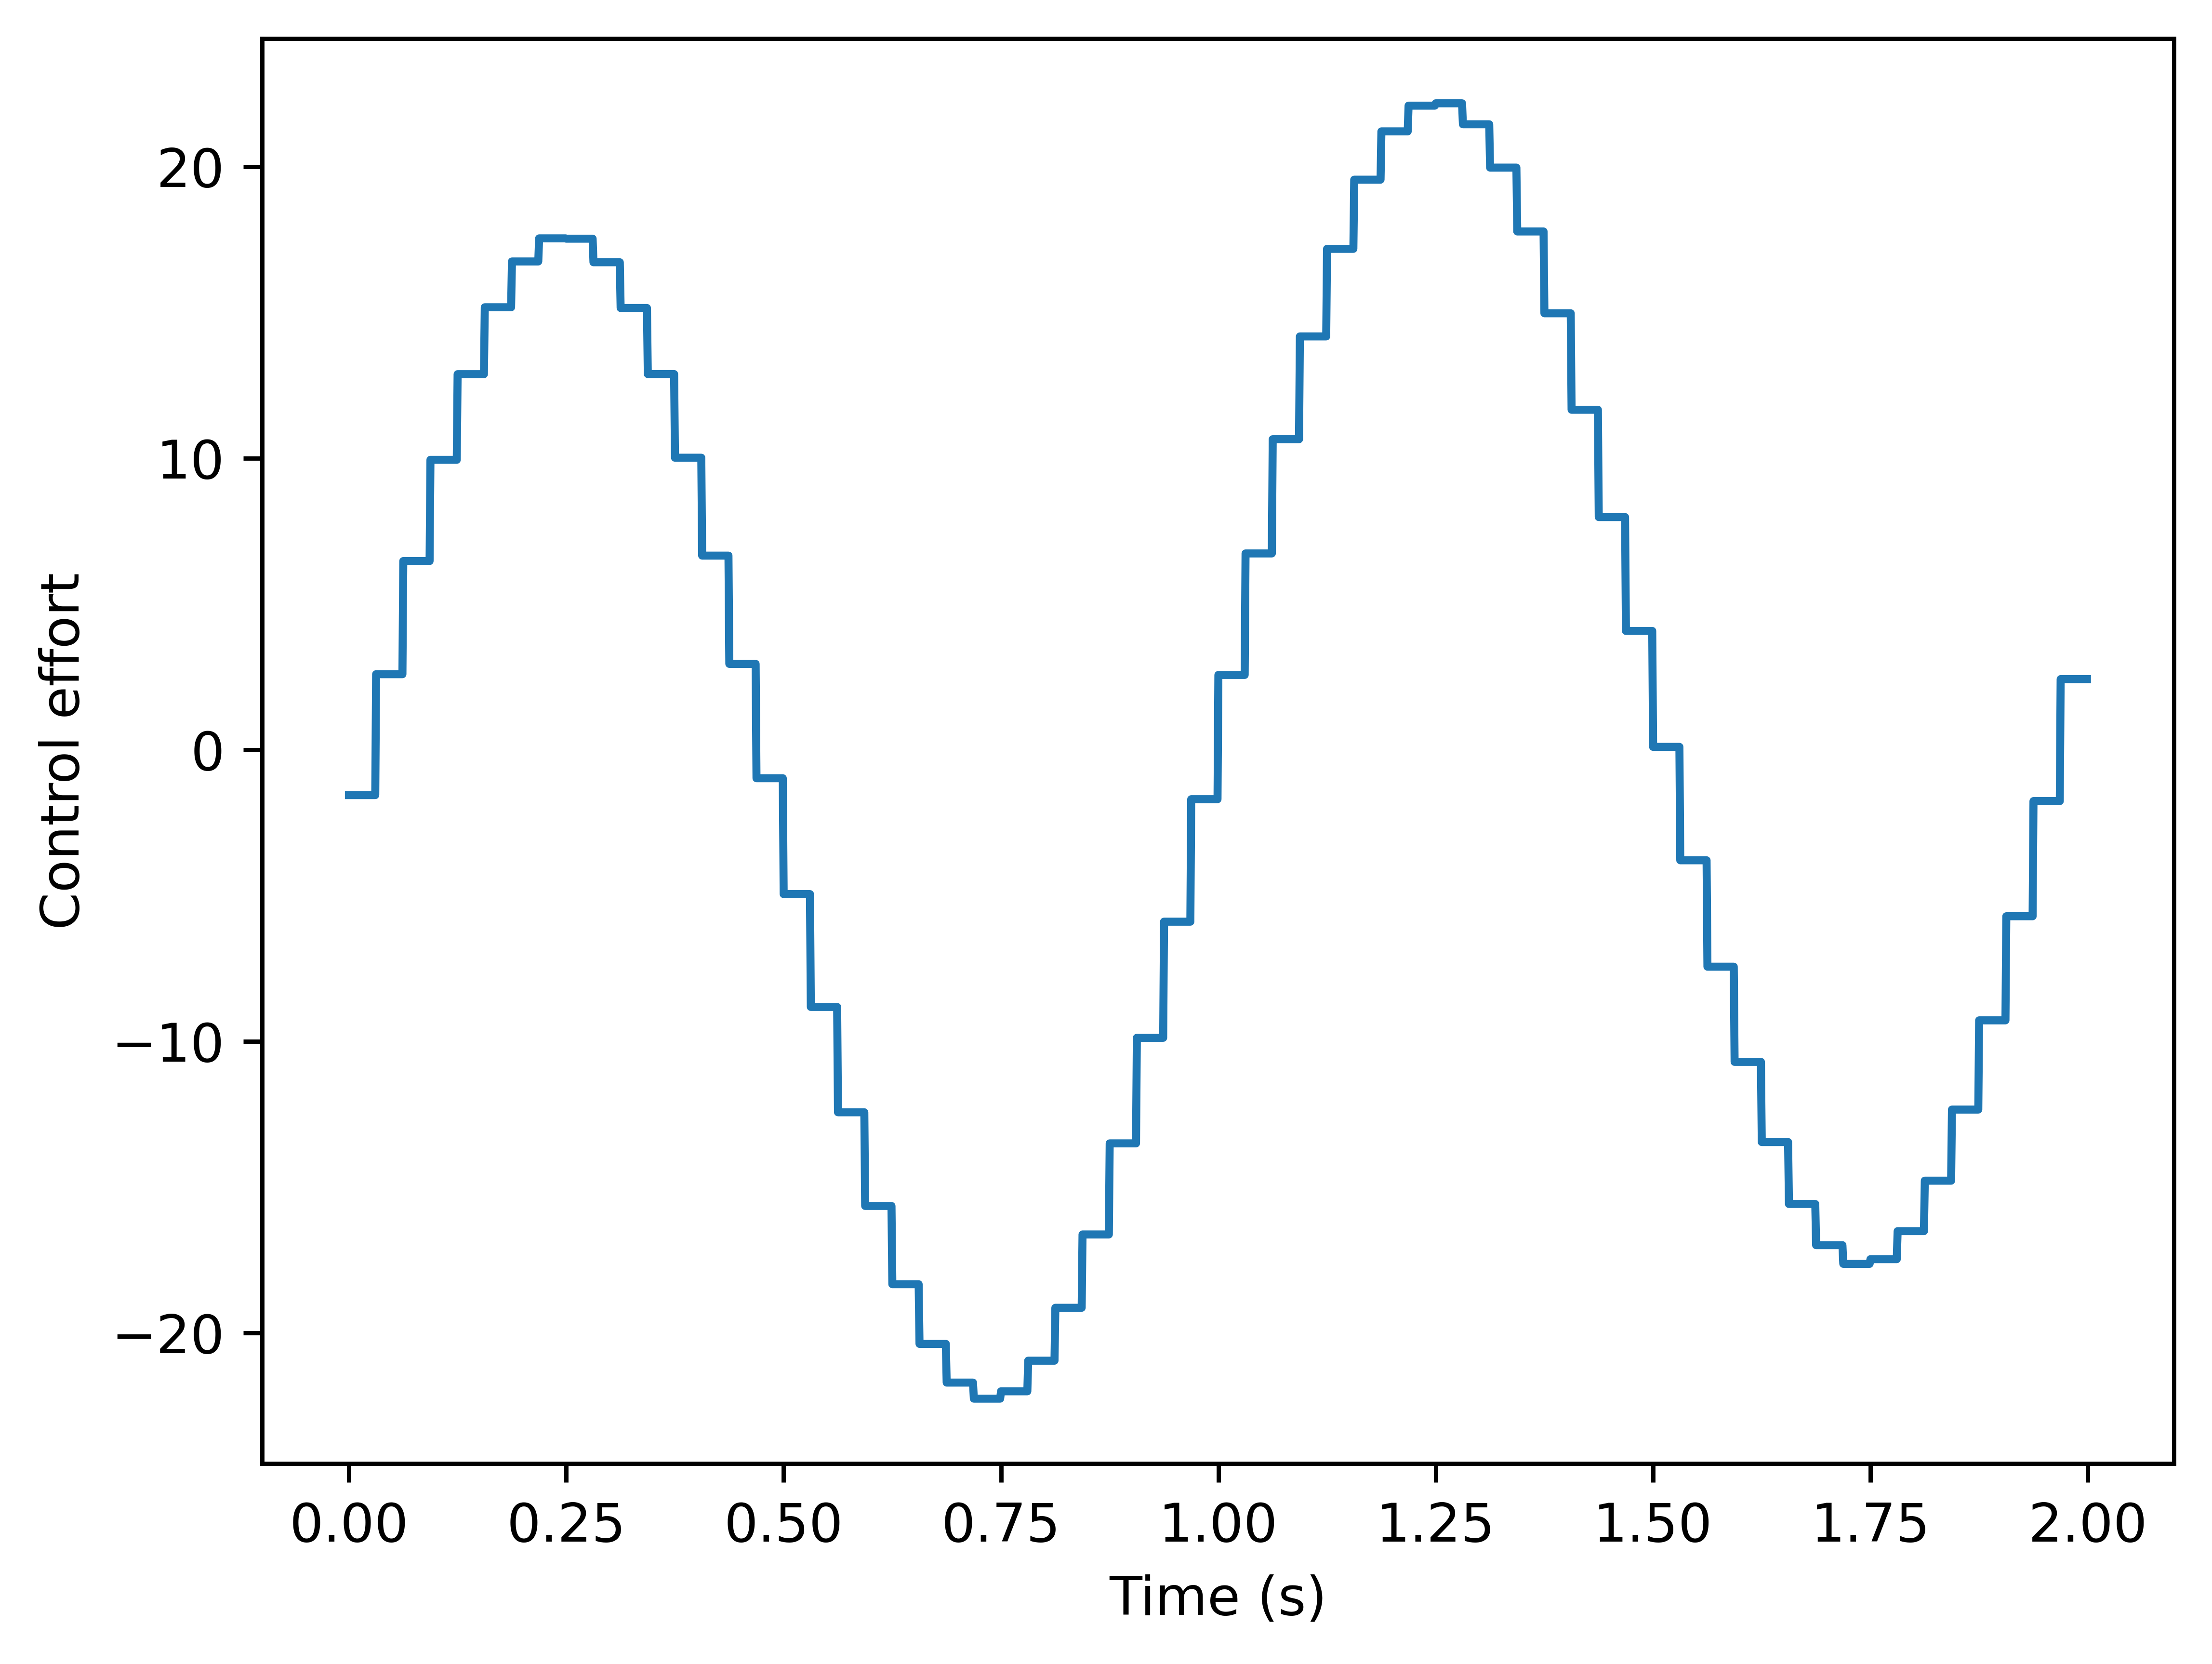
\includegraphics[width=1.0\linewidth]{control_inputty.png}
    \caption{Cartpole trajectory and control input for a cartpole swing-up scenario with $T = 2$, $N = 64$, $u \in [-30, 30]$, and final state $z = [2 \quad \pi \quad 0 \quad 0]^T$.}
    \label{fig:default-config-trajectory}
\end{figure}

\begin{figure}[H]
    \centering
    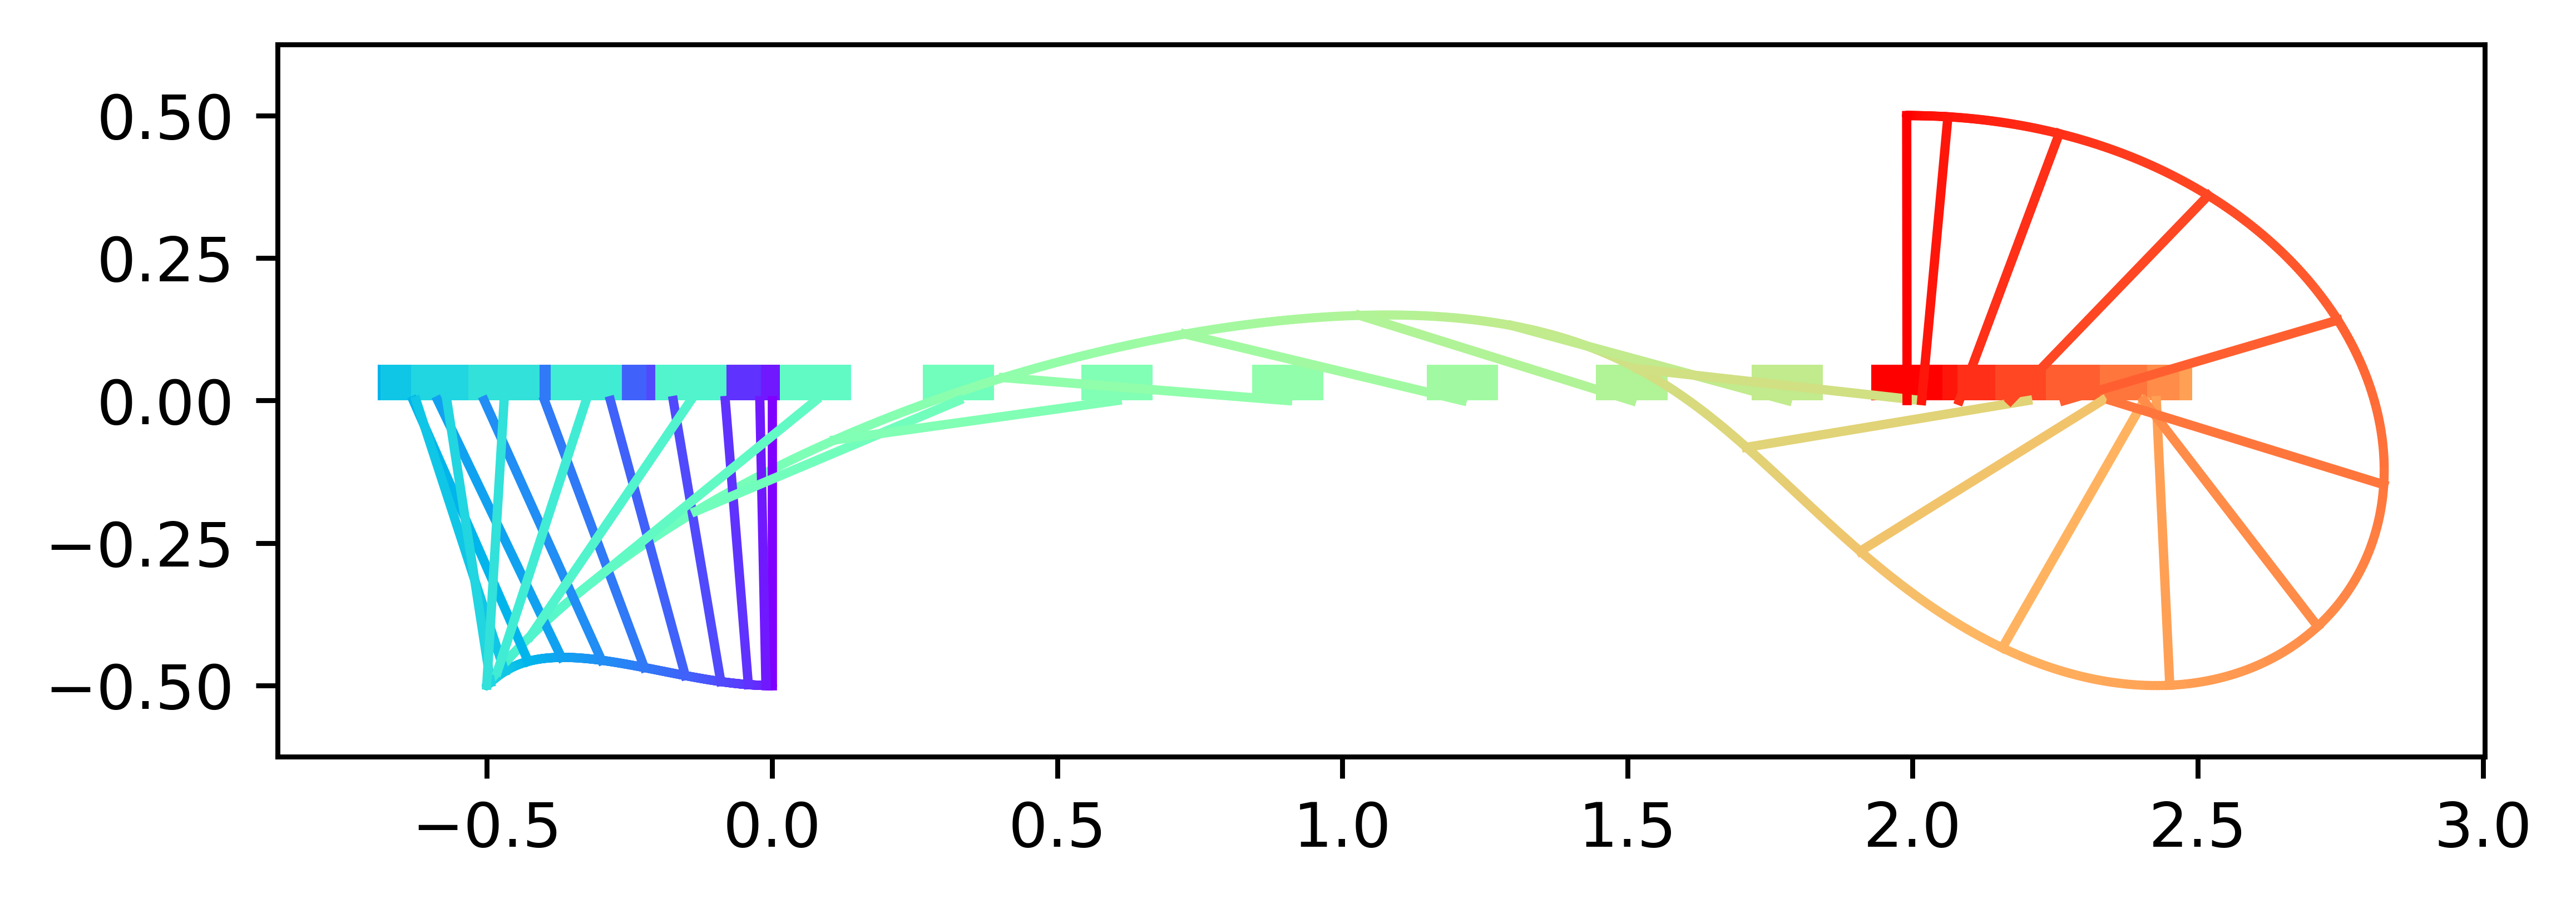
\includegraphics[width=1.0\linewidth]{cartpole_swingy-1.24s.png}
    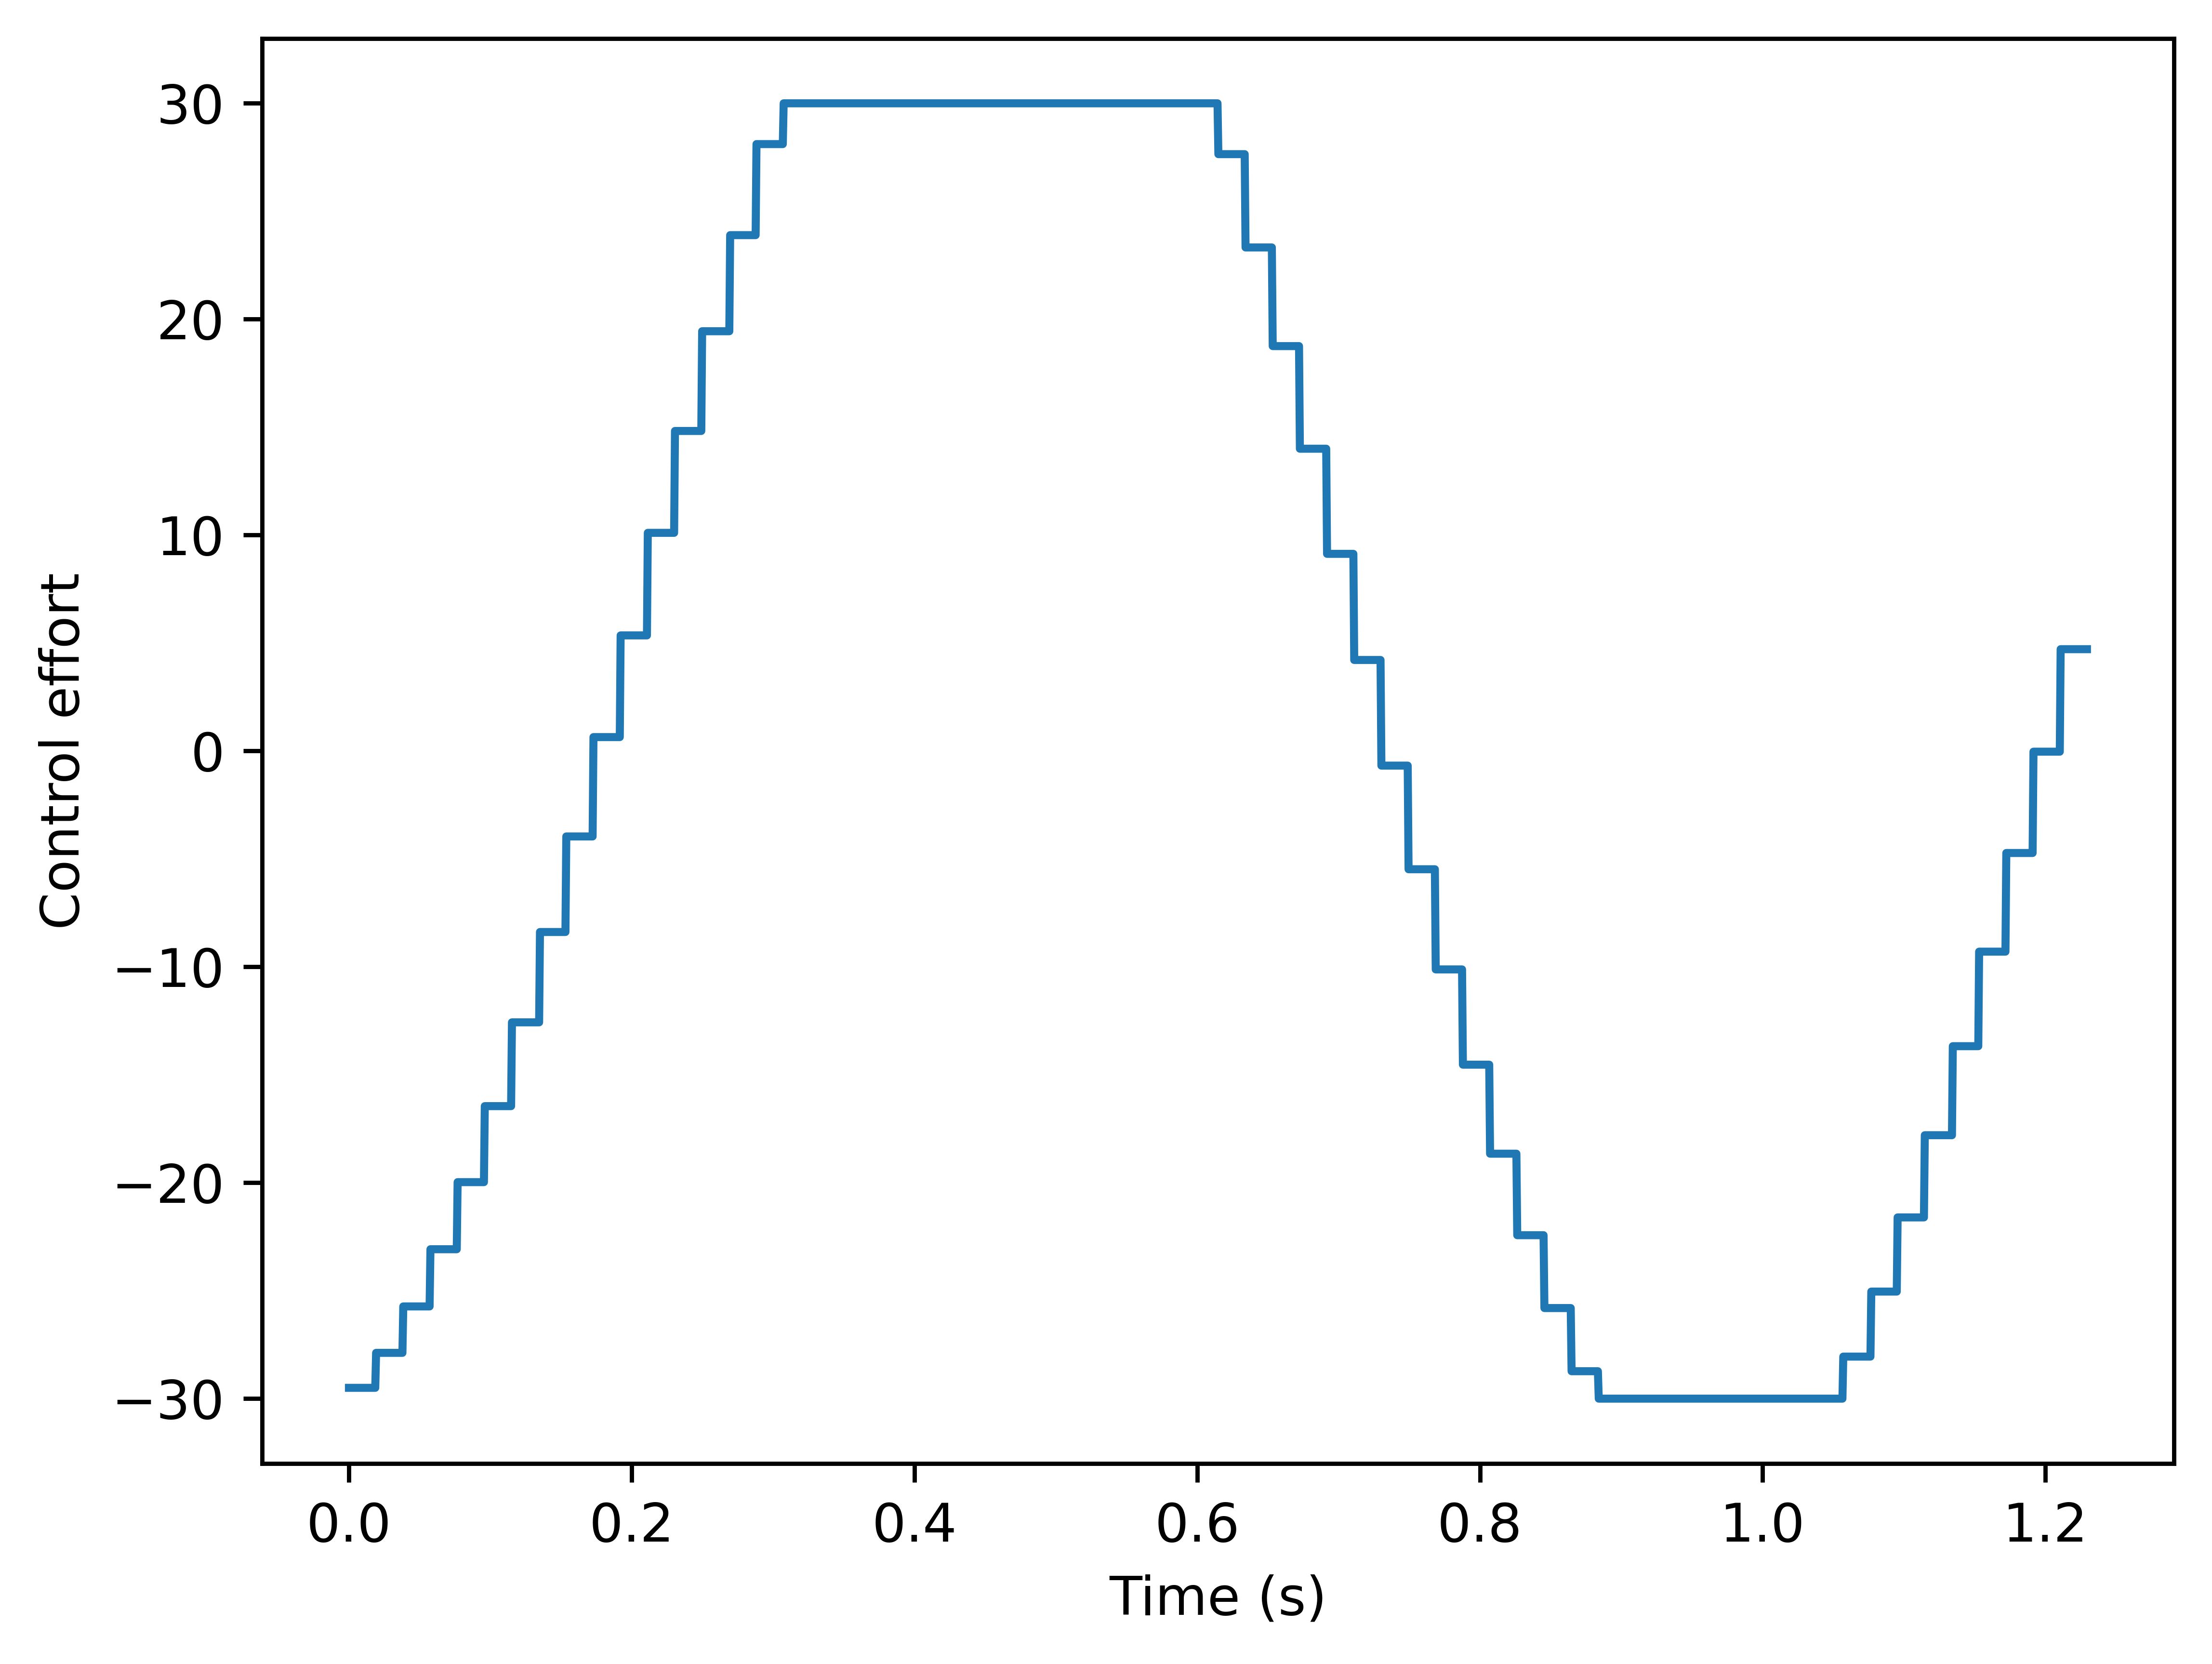
\includegraphics[width=1.0\linewidth]{control_inputty-1.24s.png}
    \caption{Cartpole trajectory and control input for a cartpole swing-up scenario with $T = 1.24$, $N = 64$, $u \in [-30, 30]$, and final state $z = [2 \quad \pi \quad 0 \quad 0]^T$.}
    \label{fig:shortest-time-trajectory}
\end{figure}

\begin{figure}[H]
    \centering
    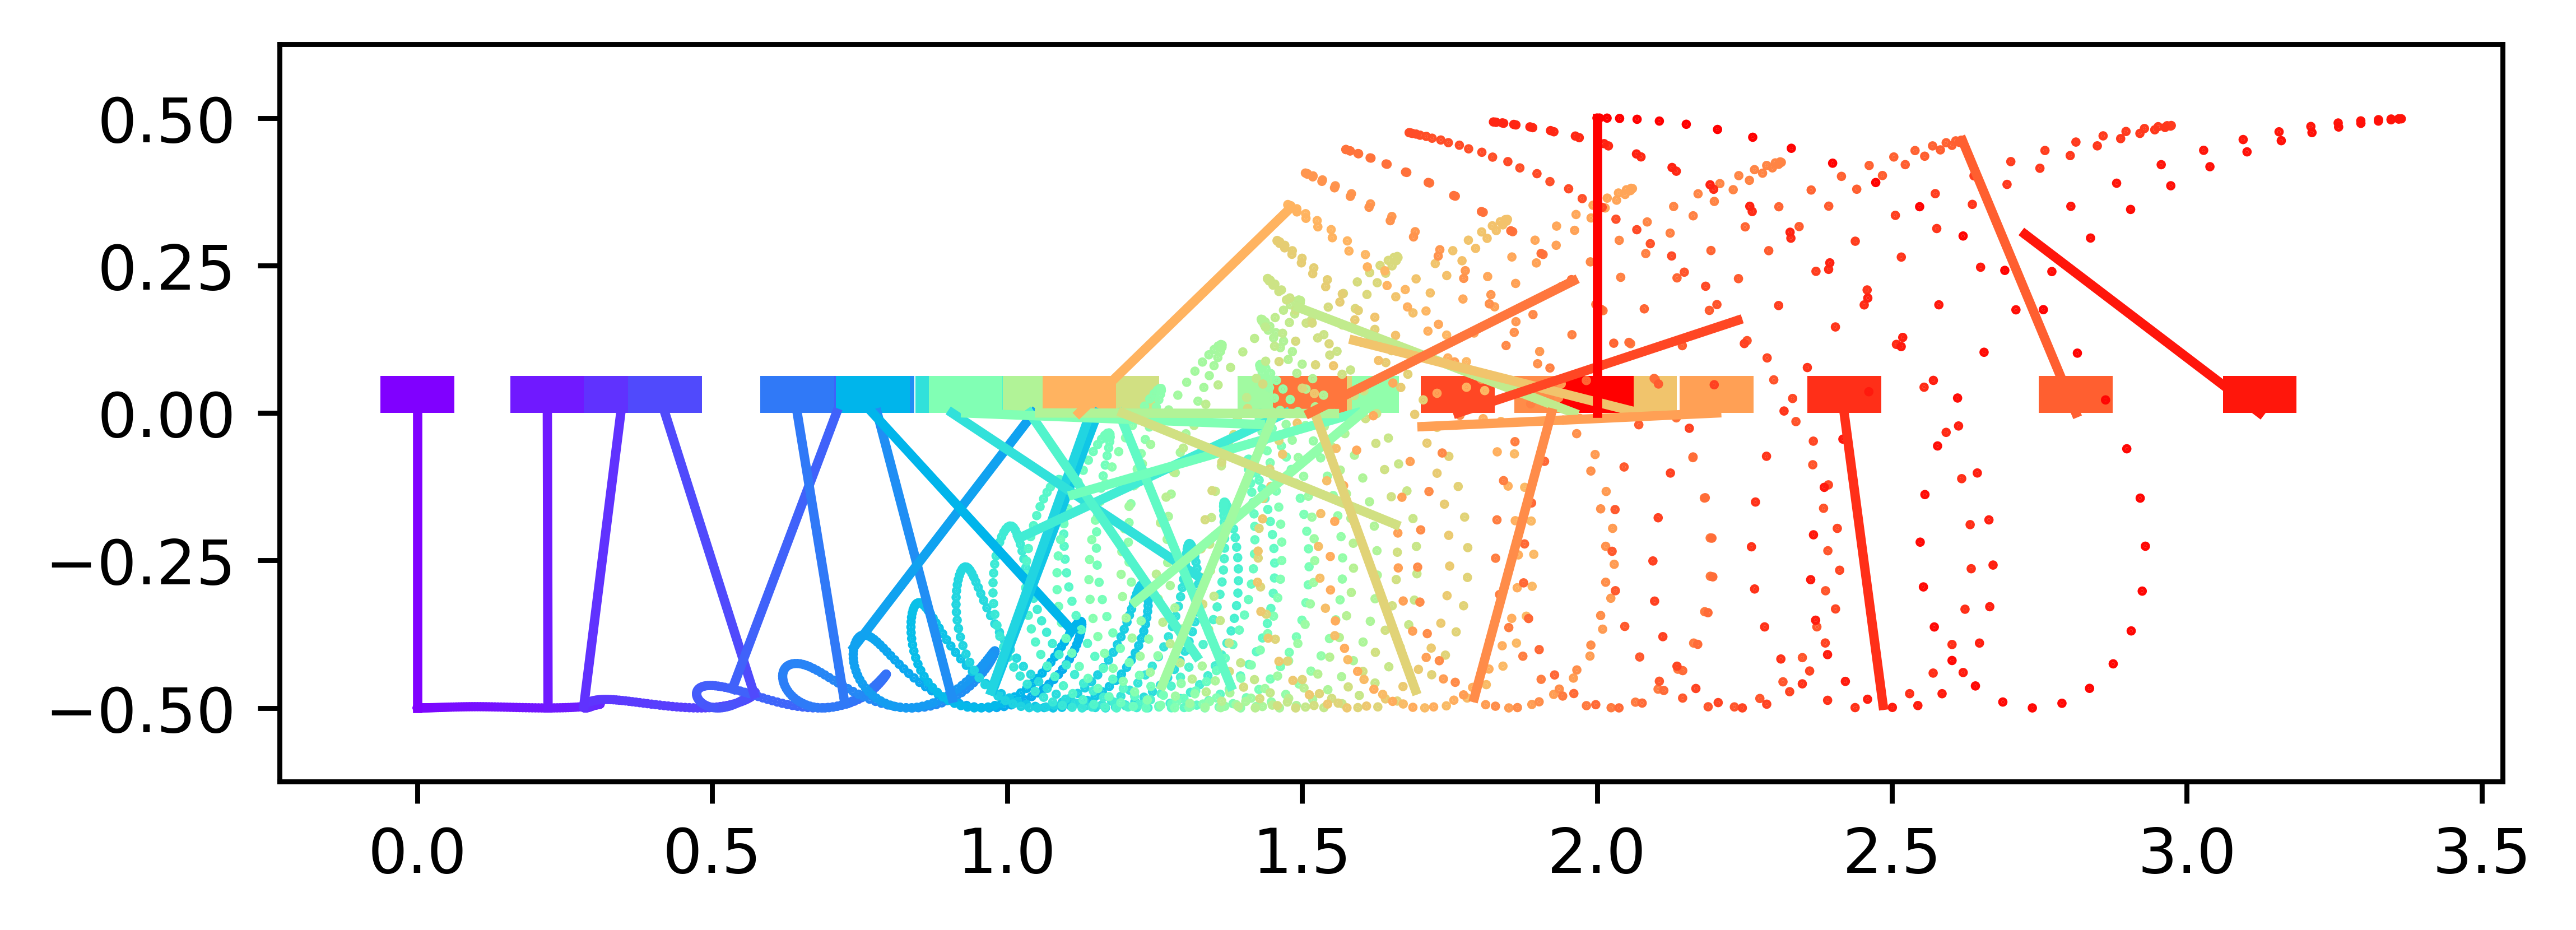
\includegraphics[width=1.0\linewidth]{default_config_T=20_N=64_z0=0.0_0.0_0.0_0.0_zf=2.0_3.141592653589793_0.0_0.0__cartpole_swingy.png}
    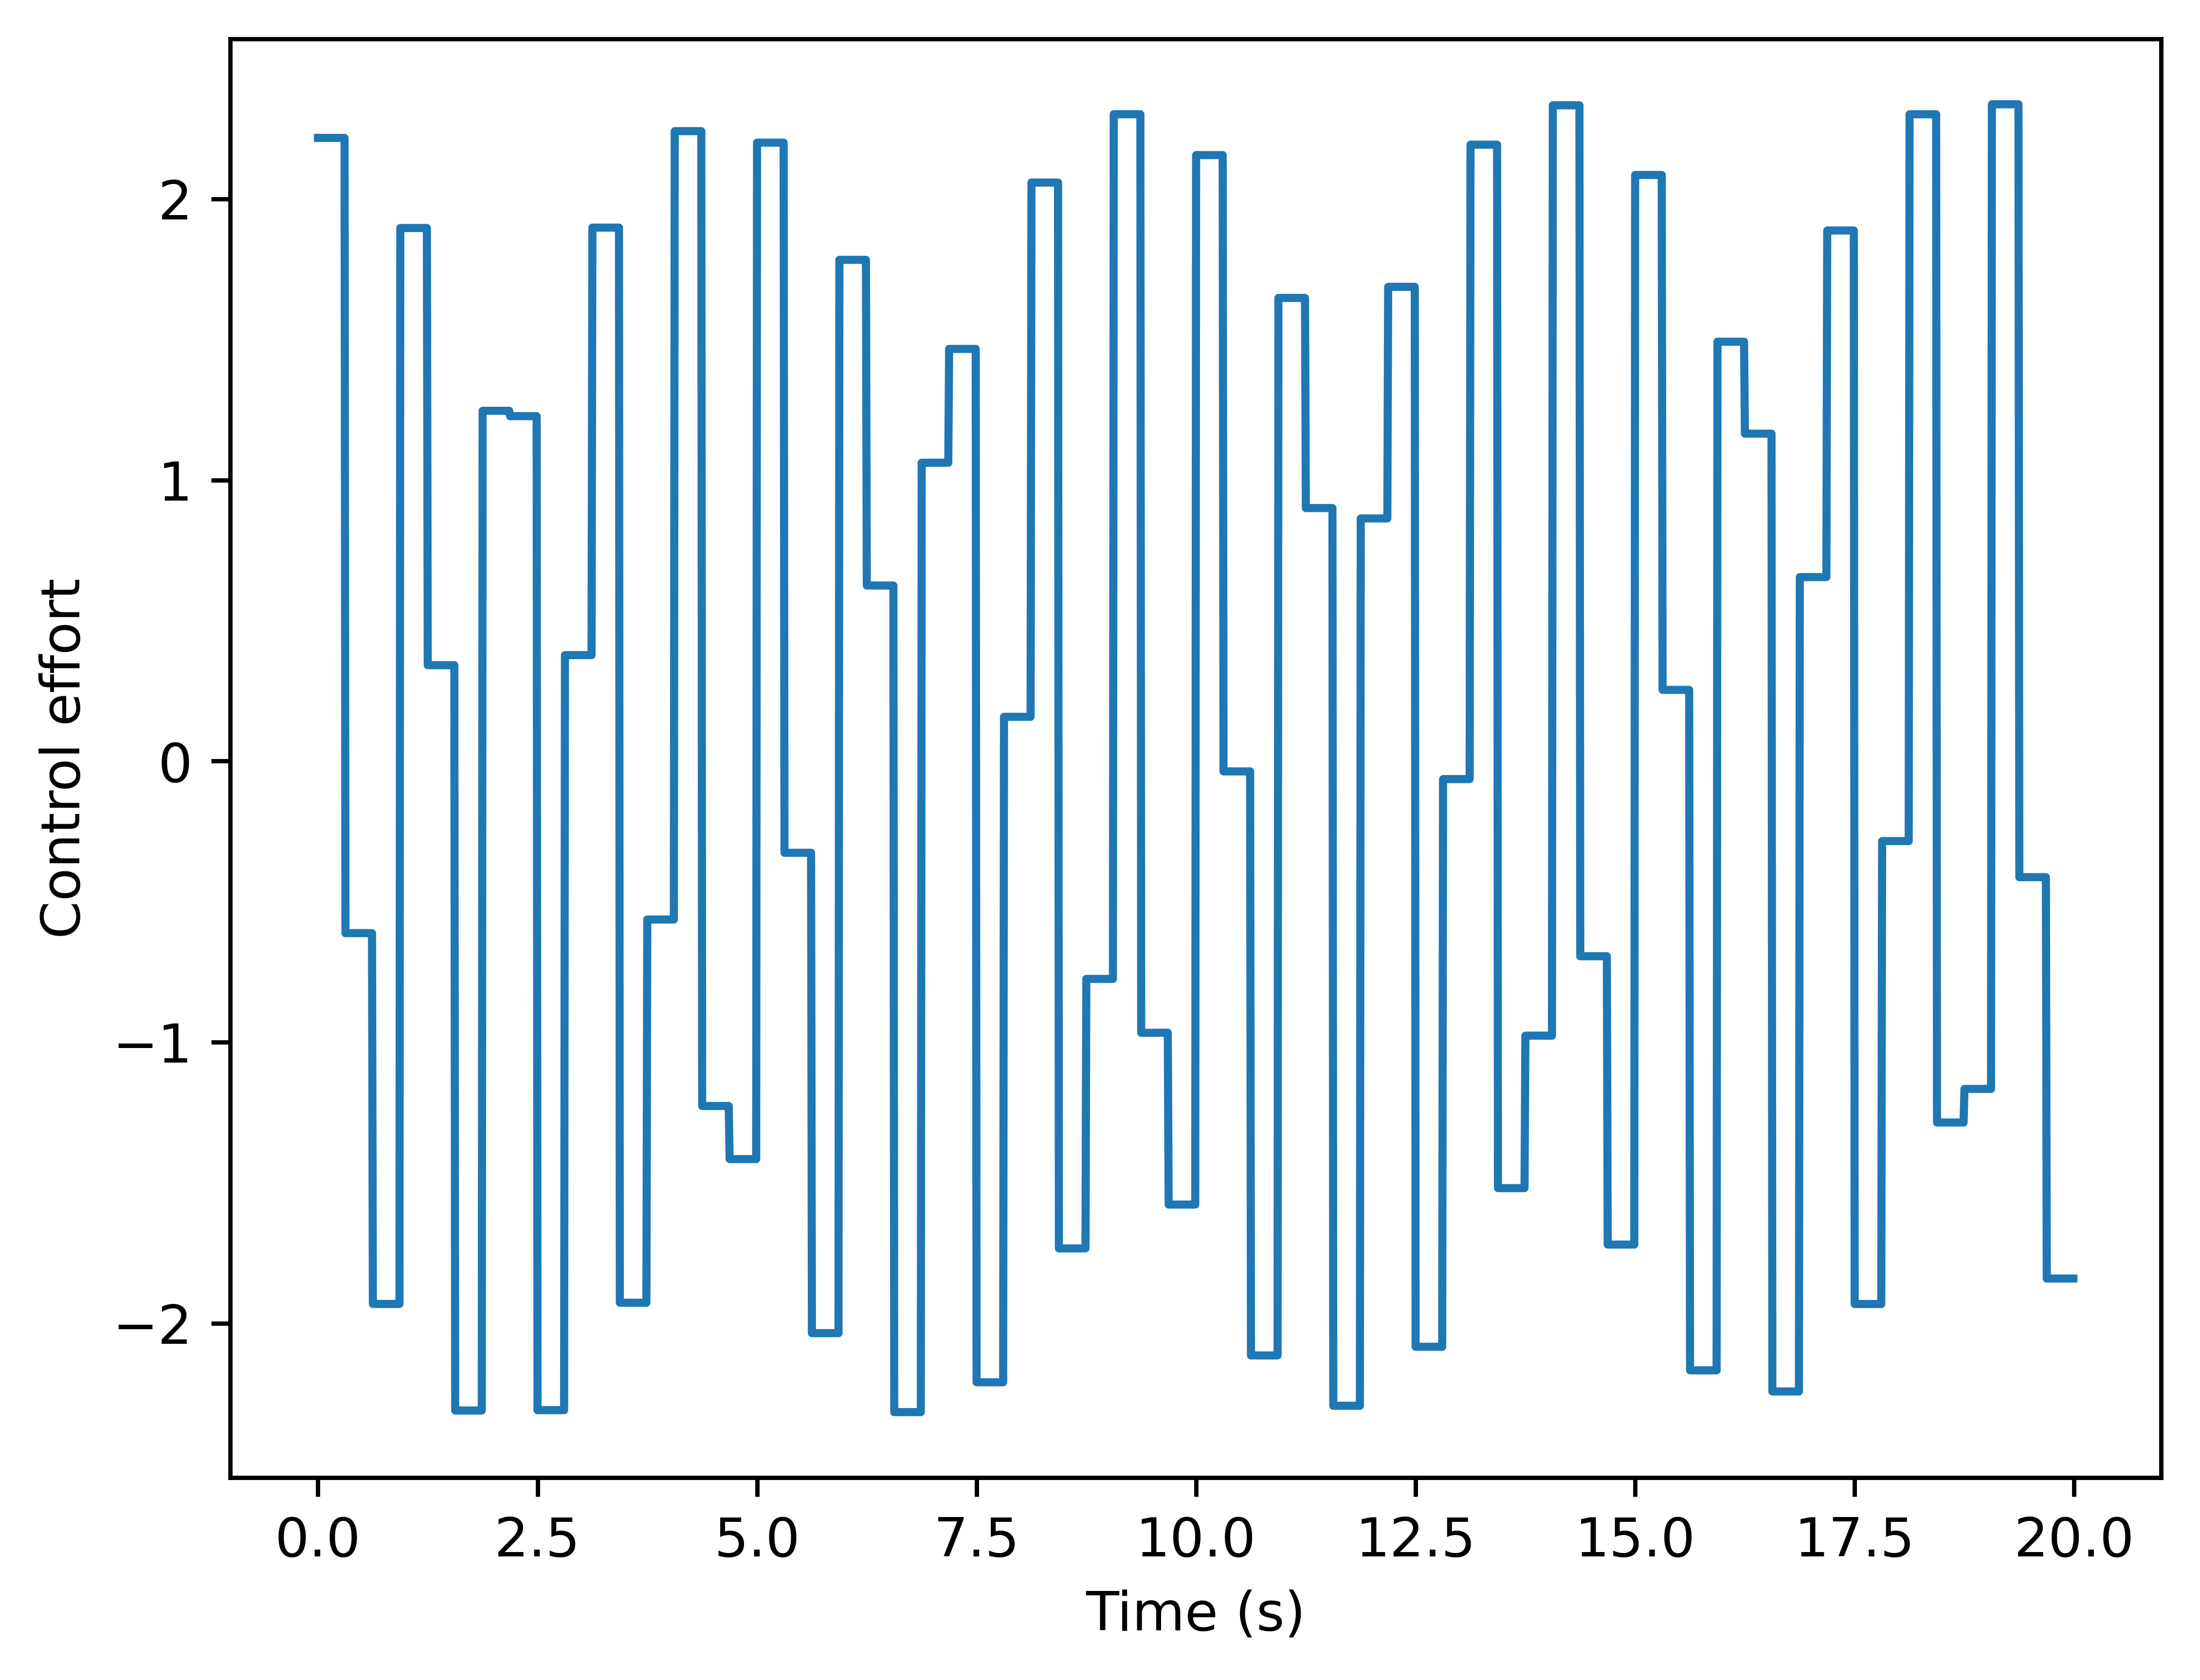
\includegraphics[width=1.0\linewidth]{default_config_T=20_N=64_z0=0.0_0.0_0.0_0.0_zf=2.0_3.141592653589793_0.0_0.0__control_inputty.png}
    \caption{Cartpole trajectory and control input for a cartpole swing-up scenario with $T = 20$, $N = 64$, $u \in [-30, 30]$, and final state $z = [2 \quad \pi \quad 0 \quad 0]^T$.}
    \label{fig:loooong-time-trajectory}
\end{figure}

\end{multicols}

\bibliographystyle{plain} % We choose the "plain" reference style
\bibliography{refs} % Entries are in the refs.bib file
\nocite{*}

\end{document}